\section{Experimental Results \& Conclusions}

Both versions of the proposed algorithm were run on 4 pattern recognition datasets, starting from a cosine wave and increasing in complexity to a distributed random shape pattern. These patterns are shown in Figure \ref{fig:datasets}. In all cases, the models were trained on a 2-hidden layer network with 50 neurons in each layer. Median thresholding produced much better results in all the cases and hence is used for all the results presented here.

The results of pruning using ground truth, first-order Taylor Series approximation and second-order Taylor Series approximation for both the variations of the proposed algorithm are shown in Figures, \ref{fig:cosine}, \ref{fig:diamond}, \ref{fig:rshape} and \ref{fig:drshape}.

It can be seen in all the cases that first-order Taylor Series expansion based pruning is a very bad approximation of the ground truth while ranking based on second-order expansion approximates the ground truth with much more accuracy. Also, it can be observed that the Iterative Re-Ranking version of the algorithm always performs better that the Single Overall Ranking version. All of these observations are in consistence with the intuitive assumptions from the Methodology section. 

Table \ref{tab:results} provides an overall summary of the experiments carried out. It can be seen that all of the experiments were carried out on optimally trained networks. The percentages shown represent the amount of pruning possible without a significant drop in performance.

In conclusion, it can be said that using the second-order Taylor Series expansion of the error function to rank individual neurons is an encouragingly accurate method of pruning networks to save memory. However it is definitely not the most accurate representation of the ranking based on the actual contribution of neurons to the error function. Another key take-away is that there are dependencies between individual neurons which might not be apparent from the outside. The better success of the Iterative Re-Ranking algorithm validates this. Perhaps a different approach like using Legendre Polynomials instead of the Taylor Series expansion would result in a better approximation of the neuron contributions.


\begin{figure}
  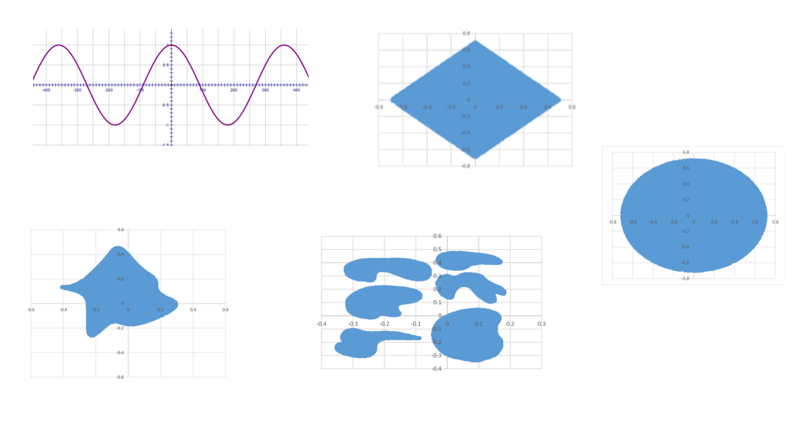
\includegraphics[width=\linewidth]{datasets.png}
  \caption{The experiments were carried out on the following patters: Cosine wave, Diamond, Random Shape, Distributed Random Shape.}
  \label{fig:datasets}
\end{figure}

\begin{figure}
  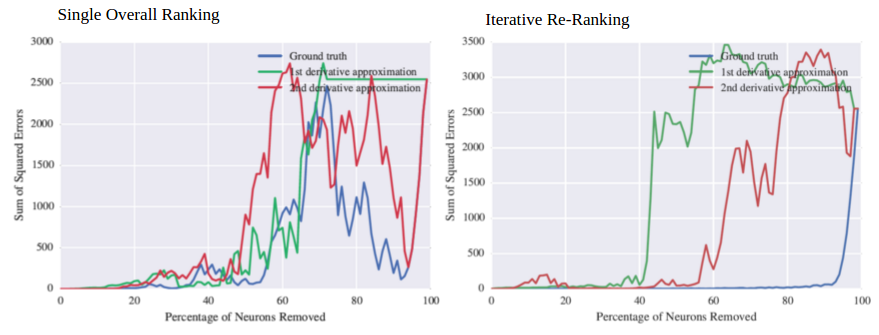
\includegraphics[width=\linewidth]{cosine.png}
  \caption{Performance on a cosine wave dataset for both variations of the proposed algorithm. The blue curve shows the ground truth estimated from brute force pruning, the green and the red curves show pruning based on the approximation from first and second-order expansion of the Taylor Series.}
  \label{fig:cosine}
\end{figure}

\begin{figure}
  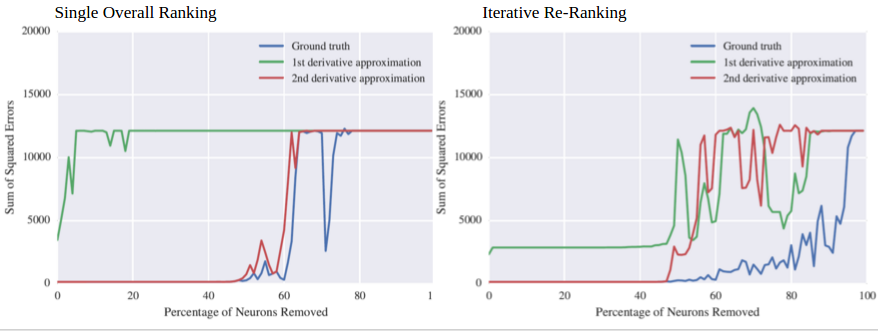
\includegraphics[width=\linewidth]{diamond.png}
  \caption{Performance on a diamond pattern dataset for both variations of the proposed algorithm. The blue curve shows the ground truth estimated from brute force pruning, the green and the red curves show pruning based on the approximation from first and second-order expansion of the Taylor Series.}
  \label{fig:diamond}
\end{figure}

\begin{figure}
  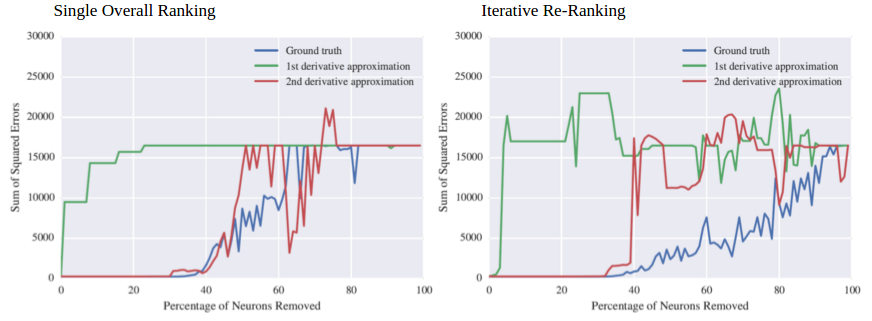
\includegraphics[width=\linewidth]{rshape.png}
  \caption{Performance on a random shape pattern dataset for both variations of the proposed algorithm. The blue curve shows the ground truth estimated from brute force pruning, the green and the red curves show pruning based on the approximation from first and second-order expansion of the Taylor Series.}
  \label{fig:rshape}
\end{figure}

\begin{figure}
  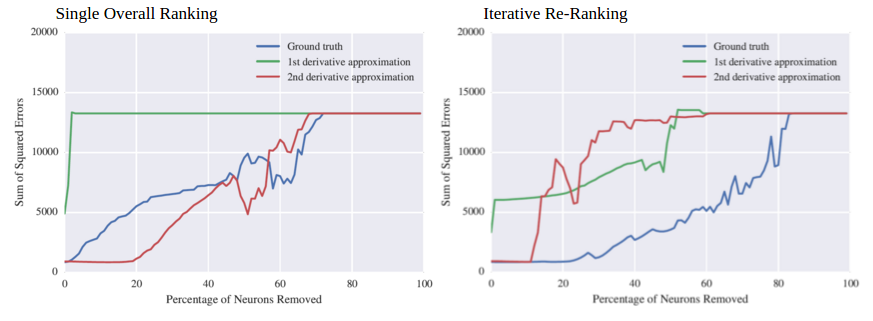
\includegraphics[width=\linewidth]{drshape.png}
  \caption{Performance on a distributed random shape pattern dataset for both variations of the proposed algorithm. The blue curve shows the ground truth estimated from brute force pruning, the green and the red curves show pruning based on the approximation from first and second-order expansion of the Taylor Series.}
  \label{fig:drshape}
\end{figure}

\begin{table}[h!]
  \begin{center}
    \begin{tabular}{c||c||c||c}
    	Pattern & Test Acc. & \ Ground Truth & Proposed Algorithm\\
    	\hline
    	\hline
      	Cosine Wave & 0.9999 & 90$\%$ & 70$\%$\\
      	\hline
      	Diamond & 0.9921 & 48$\%$ & 48$\%$\\
      	\hline 
      	Random & 0.9861 & 38$\%$ & 35$\%$\\
      	\hline 
      	Dist. Random & 0.9601 & 20$\%$ & 10$\%$\\
      	\hline
      	Circle & 0.9968 & 40$\%$ & 0$\%$\\
    \end{tabular}
  \end{center}
  \caption{A comparison of the percentage pruning achieved using brute force and the proposed algorithm on optimally trained networks. The percentages shown represent the amount of pruning possible without a significant drop in performance.}
  \label{tab:results}
\end{table}